\documentclass{article}
\usepackage[utf8]{inputenc}
\usepackage{verbatim}
\usepackage{float}
\usepackage{graphicx}
\usepackage[bottom]{footmisc}

\title{Przetwarzanie obrazu za pomocą konwolucyjnej sieci neuronowej - wyniki pracy}

\author{Józef Jasek}

\usepackage{natbib}
\usepackage{graphicx}

\begin{document}

\maketitle

\section{Wstęp teoretyczny}
\subsection{Przyjęte oznaczenia}
    Rozpatrując pojedynczą warstwę przyjmiemy następujące oznaczenia: \\
    X - wejściowa macierz danych \\
    k - liczba przykładów w wejściowej macierzy danych \\
    m - liczba neuronów warstwy poprzedniej \\
    n - liczba neuronów warstwy obecnej \\
    A - macierz wyników otrzymana po przepuszczeniu X przez warstwę \\
    Y - wyznaczone pochodne z poprzedniej warstwy lub w przypadku funkcji kosztu poprawne etykiety danych wejściowych
\subsection{Podstawa matematyczna propagacji wstecznej}
\begin{figure}[H]
    \centering
    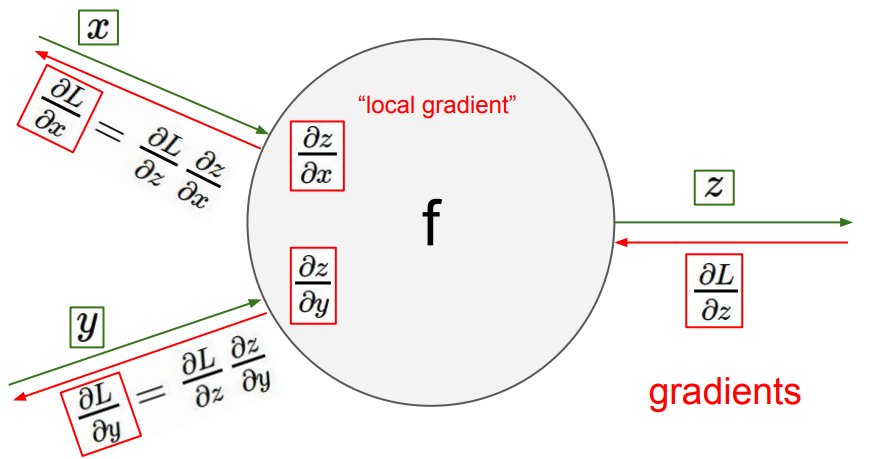
\includegraphics[width=\textwidth]{neuron.png}
    \caption{Funkcja wyjścia i pochodne funkcji kosztu po funkcjach wejścia w pojedynczym neuronie}
    \label{fig:mesh1}
\end{figure}
Do wyznaczenia pochodnych funkcji kosztu względem wag wykorzystamy zależność
\[ \frac{\partial L}{\partial x} = \frac{\partial L}{\partial z} \cdot \frac{\partial z}{\partial x} \]
Stąd możemy wyznaczyć pochodne wszystkich wag jako
\[\frac{\partial L}{\partial \omega_n}\]
\[ \frac{\partial L}{\partial \omega_{n-1}} = \frac{\partial L}{\partial x_n} \cdot \frac{\partial x_n}{\partial \omega_{n-1}} \]
\[ \frac{\partial L}{\partial \omega_{n-2}} = \frac{\partial L}{\partial x_n} \cdot \frac{\partial x_n}{\partial x_{n-1}} \cdot \frac{\partial x_{n-1}}{\partial \omega_{n-2}} \]
\[ ... \]
\[ \frac{\partial L}{\partial \omega_1} = \frac{\partial L}{\partial x_n} \cdot ... \cdot \frac{\partial x_2}{\partial \omega_1} \]
\subsection{Funkcja kosztu}
    Wykorzystywaną funkcją kosztu jest
    \[L = \frac{-1}{mk}\sum_{m,k}(Y_{m,k} \cdot log(A_{m,k} + (1 - Y) \cdot log(1 - A_{m,k})) \]
    lub w postaci macierzowej
    \[ L = -Avg(Y \cdot log(A) + (1 - Y) log(1 - A)) \]
    Możemy teraz wyznaczyć niezbędne pochodne do algorytmu wstecznej propagacji
    \[ \frac{\partial L}{\partial A} = \frac{-1}{mk}\left(\frac{Y}{A} - \frac{1 - Y}{1 - A}\right) =
        \frac{-1}{mk}\left( \frac{Y(1 - A) - A(1 - Y)}{A(1 - A)} \right) = 
        \frac{-1}{mk}\left( \frac{Y - A}{A - A^2} \right)\]
    Ponieważ $mk$ jest stałą możemy ją pominąć rekompensując odpowiednio zmienionym hiperparametrem $\alpha$. Otrzymujemy więc
    \[ \frac{\partial L}{\partial A} = -\frac{Y - A}{A - A^2} \]
\subsection{Sigmoida}
    Sigmoida dana jest wzorem
    \[ A = \frac{1}{1 + e^{-x}} \]
    
    Wzór używany w propagacji wstecznej to
    \[ \frac{\partial A}{\partial X} = \frac{e^{-x}}{(1 + e^{-x})^2} \]
    
\subsection{Softmax}
    Funkcja softmax dana jest wzorem
    \[ A_j = \frac{e^{X_j}}{\sum_{i=1}^m e^{X_i}} \]
    
    Wzór używany w propagacji wstecznej to
    \[ \frac{\partial A_i}{\partial X_j} = 
    \left\{
        \begin{array}{ll}
        A_i(1 - A_j) & \mbox{dla } i = j \\
        -A_iA_j & \mbox{dla } i \neq j
        \end{array}
    \right. \]

\subsection{Konwolucja}
\begin{figure}[H]
    \centering
    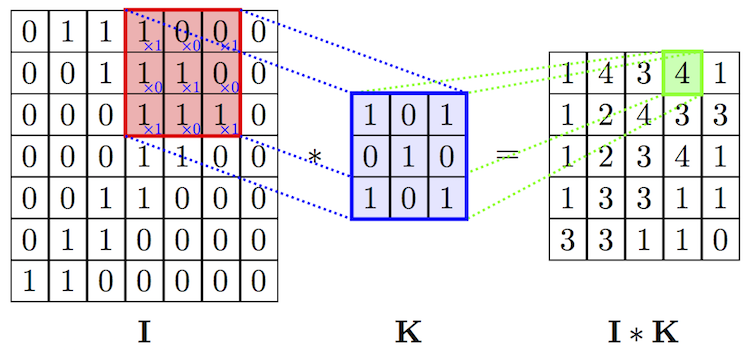
\includegraphics[width=\textwidth]{convolution.png}
    \caption{Warstwa konwolucyjna}
    \label{fig:mesh1}
\end{figure}
W przypadku warstwy konwolucyjnej zamiast po prostu mnożyć element wejściowy przed wagę, wykorzystujemy filtry małej wielkości, którymi wielokrotnie przejeżdżamy po naszym wejściu i dla każdego fragmentu stosujemy mnożenie macierzy po elementach. Każdy filtr generuje jedno dwuwymiarowe przekształcenie danych wejściowych. Po obliczeniu konwolucji transformujemy wynik funkcją sigmoidalną wg wzoru jak wyżej.

\subsection{Maxpool}
\begin{figure}[H]
    \centering
    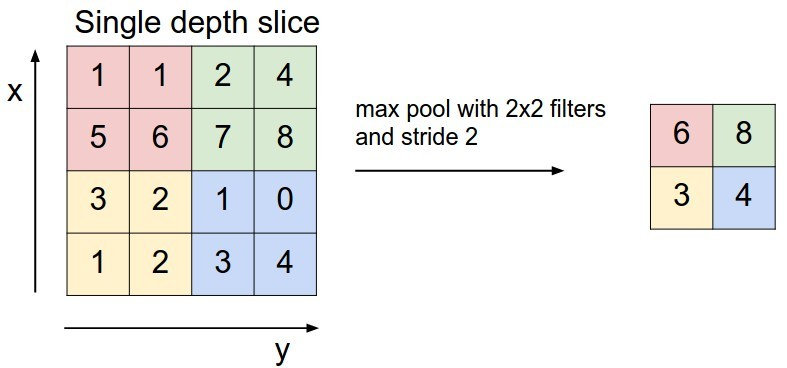
\includegraphics[width=\textwidth]{maxpool.jpeg}
    \caption{Warstwa maxpool}
    \label{fig:mesh1}
\end{figure}
Warstwa maxpool działa jak warstwa konwolucyjna, ale zamiast nakładać filtr wybiera element maksymalny z danego fragmentu i podaje go na wyjściu. Przy propagacji wstecznej ten element, który został wybrany ma pochodną równą pochodnej wyjścia, a pozostałe pochodne są równe 0.

\begin{comment}
\subsection{Funkcja sigmoidalna}
    \[ A = \frac{1}{1 + exp(-(W^T * X + B)^T)} \]
    \[ \frac{\partial A}{\partial W} =  \]
  dw = ((*lastX) * activatedWeights.dot(-activatedWeights + 1).dot(prevError)) / prevError.get_rows();

\end{comment}
\section{Model sieci}
Wstępnie zaproponowany model sieci przedstawia się następująco
\begin{figure}[H]
\makebox[\textwidth][c]{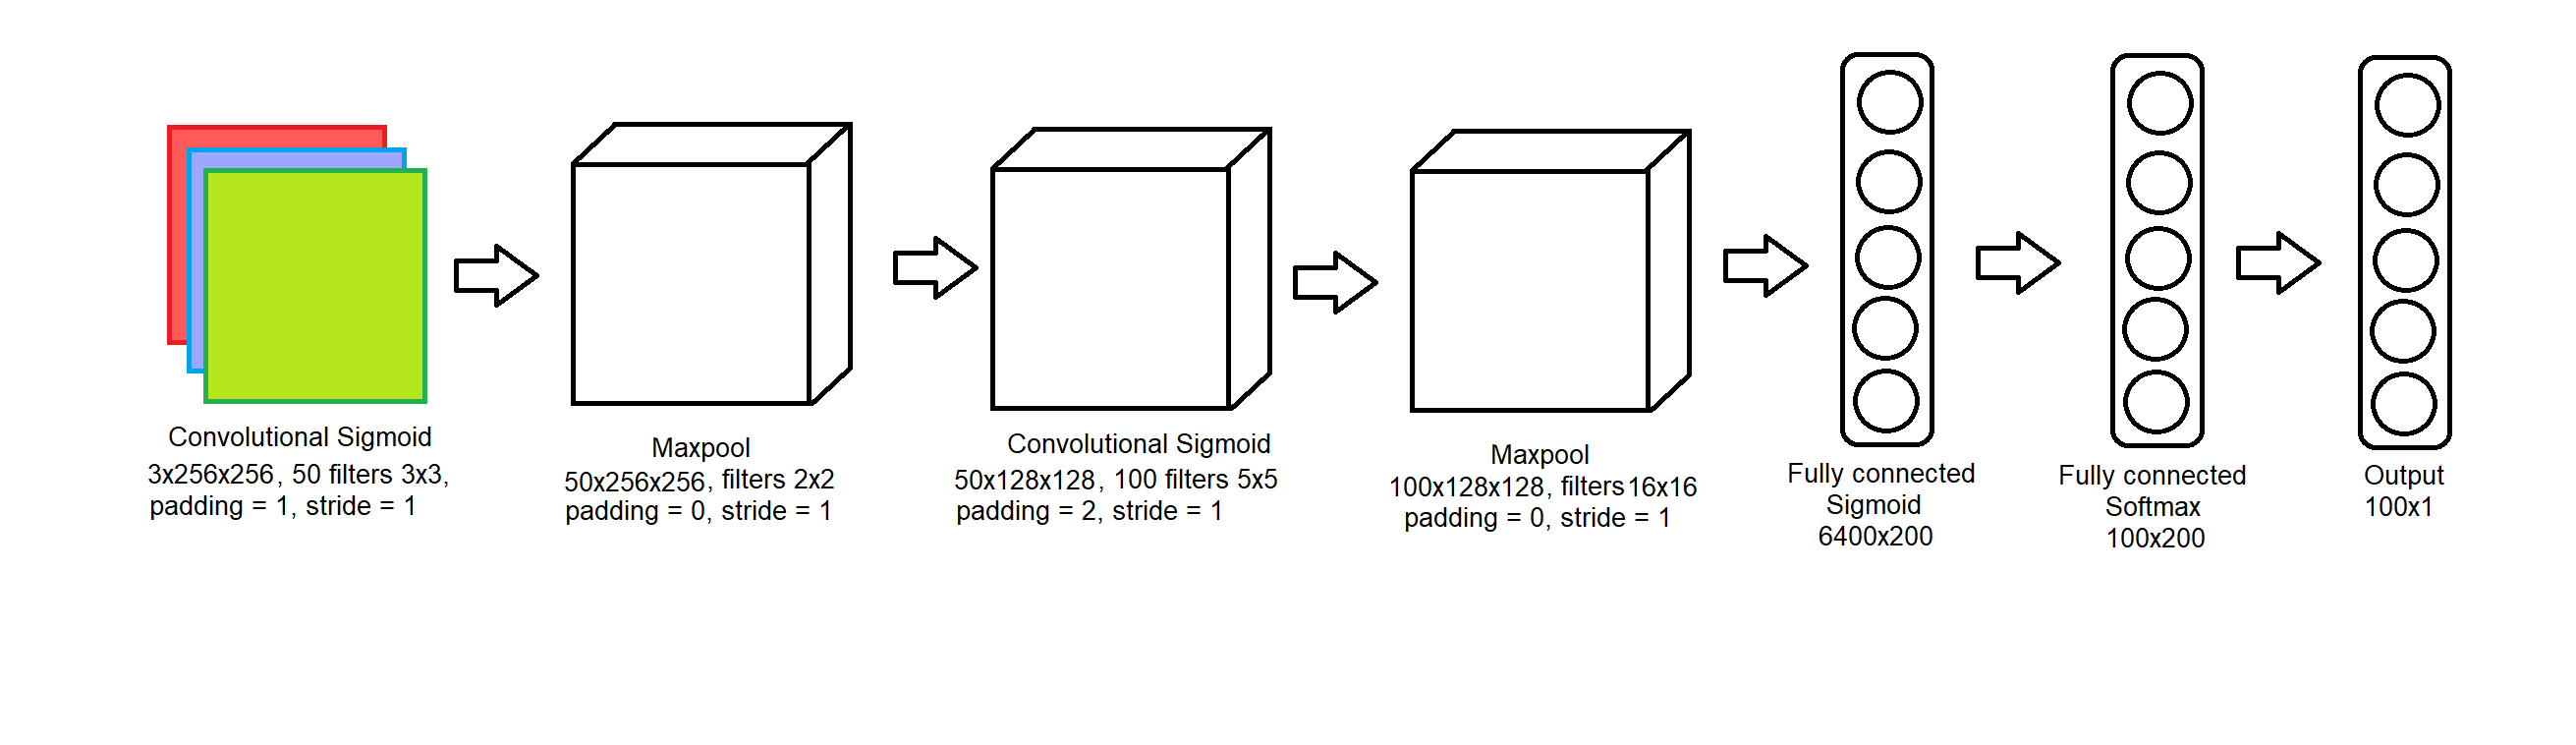
\includegraphics[width=1.7\textwidth]{nn.png}}%
\centering
\caption{Proponowany model sieci}
\end{figure}


\section{Implementacja}
W ramach realizacji projektu zaimplementowano w C++ następujące elementy uczenia maszynowego
\begin{itemize}
    \item implementacja dwuwymiarowych macierzy (podstawowe operacje matematyczne, operacje per element, transpozycja, zapisywanie do strumienia danych, inicjalizacja wartości wg rozkładu Gaussa, funkcja sigmoidalna, eksponenta, logarytm per element, suma po wybranych wymiarach)
    \item warstwa fully-connected sieci neuronowej nakładająca funkcję sigmoidalną z operacjami propagacji wprzód i wstecz, inicjalizacją wartości wg rozkładu Gaussa, aktualizacją wag na podstawie propagacji wstecz, zapisywanie wag do strumienia danych)
    \item warstwa softmax ze wszystkimi elementami jak wyżej
    \item warstwa maxpool i konwolucyjna ze wszystkimi elementami jak wyżej oraz dodatkowo operacją transformacji 4-wymiarowego inputu/outputu warstwy konwolucyjnej na 2-wymiarowy input/output warstwy w pełni połączonej
    \item testy jednostkowe do wszystkich wyżej wymienionych elementów
\end{itemize}
Dodatkowo w ramach obróbki analizowanych zdjęć zaimplementowano w języku Python
\begin{itemize}
    \item generator obrazów zawierających słowa z listy top 100 słów w języku angielskim z możliwością transformacji przez obrót, skalowanie, zmiana koloru czcionki i tła, zmiana rodziny czcionki i jej rozmiaru
    \item program do wyświetlania i analizy wyjść warstwy konwolucyjnej
\end{itemize}
\section{Realizacja}
Po zaimplementowaniu sieci do trenowania użyliśmy 10 najpopularniejszych słów zamiast 100 ze względu na duże narzuty pamięciowe, które uniemożliwiły trenowanie większej liczby słów na naszym modelu. Nasza próbka danych treningowych wyniosła 180 obrazków. Z uwagi na fakt, że nie udało się zrealizować projektu do końca, nie zdążyliśmy stworzyć zbioru danych testowych. Trenowanie trwało 150 epok. Po trenowaniu i przetestowaniu outputu sieci neuronowej mogliśmy zauważyć, że zwraca ona $10\%$ prawdopodobieństwo przynależności do każdej klasy dla każdego obrazka.
\section{Podsumowanie}
Niestety przez zastosowanie funkcji sigmoidalnej w naszej sieci doszło do tzw. problemu znikającego gradientu. Już przy czwartej warstwie gradient zwracany przez propagację wsteczną był na poziomie błędu reprezentacji zmiennoprzecinkowej skutecznie uniemożliwiając poprawne wytrenowanie sieci. Przypuszczamy, że użycie np. warstwy ReLU (Rectified Linear Unit) cechującej się stałym gradientem dla wartości dodatnich pozwoliłoby zniwelować problem, niestety zabrakło czasu na jej implementację.
\section{Bibliografia}
\begin{itemize}
    \item\begin{verbatim}https://en.wikipedia.org/wiki/Vanishing_gradient_problem\end{verbatim}
    \item\begin{verbatim}https://bit.ly/2s6lZto\end{verbatim}
    \item\begin{verbatim}https://www.researchgate.net\end{verbatim}
    \item\begin{verbatim}https://www.youtube.com/watch?v=d14TUNcbn1k\end{verbatim}
    \item\begin{verbatim}https://www.youtube.com/watch?v=bNb2fEVKeEo\end{verbatim}
    \item\begin{verbatim}https://www.coursera.org/learn/machine-learning\end{verbatim}
    \item\begin{verbatim}https://www.coursera.org/specializations/deep-learning\end{verbatim}
    
\end{itemize}
\end{document}










